\chapter{Number 34 and Number 27}

Dantès passed through all the stages of torture natural to prisoners in
suspense. He was sustained at first by that pride of conscious
innocence which is the sequence to hope; then he began to doubt his own
innocence, which justified in some measure the governor’s belief in his
mental alienation; and then, relaxing his sentiment of pride, he
addressed his supplications, not to God, but to man. God is always the
last resource. Unfortunates, who ought to begin with God, do not have
any hope in him till they have exhausted all other means of
deliverance.

Dantès asked to be removed from his present dungeon into another, even
if it were darker and deeper, for a change, however disadvantageous,
was still a change, and would afford him some amusement. He entreated
to be allowed to walk about, to have fresh air, books, and writing
materials. His requests were not granted, but he went on asking all the
same. He accustomed himself to speaking to the new jailer, although the
latter was, if possible, more taciturn than the old one; but still, to
speak to a man, even though mute, was something. Dantès spoke for the
sake of hearing his own voice; he had tried to speak when alone, but
the sound of his voice terrified him.

Often, before his captivity, Dantès’ mind had revolted at the idea of
assemblages of prisoners, made up of thieves, vagabonds, and murderers.
He now wished to be amongst them, in order to see some other face
besides that of his jailer; he sighed for the galleys, with the
infamous costume, the chain, and the brand on the shoulder. The
galley-slaves breathed the fresh air of heaven, and saw each other.
They were very happy.

He besought the jailer one day to let him have a companion, were it
even the mad abbé. The jailer, though rough and hardened by the
constant sight of so much suffering, was yet a man. At the bottom of
his heart he had often had a feeling of pity for this unhappy young man
who suffered so; and he laid the request of number 34 before the
governor; but the latter sapiently imagined that Dantès wished to
conspire or attempt an escape, and refused his request. Dantès had
exhausted all human resources, and he then turned to God.

All the pious ideas that had been so long forgotten, returned; he
recollected the prayers his mother had taught him, and discovered a new
meaning in every word; for in prosperity prayers seem but a mere medley
of words, until misfortune comes and the unhappy sufferer first
understands the meaning of the sublime language in which he invokes the
pity of heaven! He prayed, and prayed aloud, no longer terrified at the
sound of his own voice, for he fell into a sort of ecstasy. He laid
every action of his life before the Almighty, proposed tasks to
accomplish, and at the end of every prayer introduced the entreaty
oftener addressed to man than to God: “Forgive us our trespasses as we
forgive them that trespass against us.” Yet in spite of his earnest
prayers, Dantès remained a prisoner.

Then gloom settled heavily upon him. Dantès was a man of great
simplicity of thought, and without education; he could not, therefore,
in the solitude of his dungeon, traverse in mental vision the history
of the ages, bring to life the nations that had perished, and rebuild
the ancient cities so vast and stupendous in the light of the
imagination, and that pass before the eye glowing with celestial colors
in Martin’s Babylonian pictures. He could not do this, he whose past
life was so short, whose present so melancholy, and his future so
doubtful. Nineteen years of light to reflect upon in eternal darkness!
No distraction could come to his aid; his energetic spirit, that would
have exalted in thus revisiting the past, was imprisoned like an eagle
in a cage. He clung to one idea—that of his happiness, destroyed,
without apparent cause, by an unheard-of fatality; he considered and
reconsidered this idea, devoured it (so to speak), as the implacable
Ugolino devours the skull of Archbishop Roger in the Inferno of Dante.

Rage supplanted religious fervor. Dantès uttered blasphemies that made
his jailer recoil with horror, dashed himself furiously against the
walls of his prison, wreaked his anger upon everything, and chiefly
upon himself, so that the least thing,—a grain of sand, a straw, or a
breath of air that annoyed him, led to paroxysms of fury. Then the
letter that Villefort had showed to him recurred to his mind, and every
line gleamed forth in fiery letters on the wall like the \textit{mene, mene,
tekel upharsin} of Belshazzar. He told himself that it was the enmity
of man, and not the vengeance of Heaven, that had thus plunged him into
the deepest misery. He consigned his unknown persecutors to the most
horrible tortures he could imagine, and found them all insufficient,
because after torture came death, and after death, if not repose, at
least the boon of unconsciousness.

By dint of constantly dwelling on the idea that tranquillity was death,
and if punishment were the end in view other tortures than death must
be invented, he began to reflect on suicide. Unhappy he, who, on the
brink of misfortune, broods over ideas like these!

Before him is a dead sea that stretches in azure calm before the eye;
but he who unwarily ventures within its embrace finds himself
struggling with a monster that would drag him down to perdition. Once
thus ensnared, unless the protecting hand of God snatch him thence, all
is over, and his struggles but tend to hasten his destruction. This
state of mental anguish is, however, less terrible than the sufferings
that precede or the punishment that possibly will follow. There is a
sort of consolation at the contemplation of the yawning abyss, at the
bottom of which lie darkness and obscurity.

Edmond found some solace in these ideas. All his sorrows, all his
sufferings, with their train of gloomy spectres, fled from his cell
when the angel of death seemed about to enter. Dantès reviewed his past
life with composure, and, looking forward with terror to his future
existence, chose that middle line that seemed to afford him a refuge.

“Sometimes,” said he, “in my voyages, when I was a man and commanded
other men, I have seen the heavens overcast, the sea rage and foam, the
storm arise, and, like a monstrous bird, beating the two horizons with
its wings. Then I felt that my vessel was a vain refuge, that trembled
and shook before the tempest. Soon the fury of the waves and the sight
of the sharp rocks announced the approach of death, and death then
terrified me, and I used all my skill and intelligence as a man and a
sailor to struggle against the wrath of God. But I did so because I was
happy, because I had not courted death, because to be cast upon a bed
of rocks and seaweed seemed terrible, because I was unwilling that I, a
creature made for the service of God, should serve for food to the
gulls and ravens. But now it is different; I have lost all that bound
me to life, death smiles and invites me to repose; I die after my own
manner, I die exhausted and broken-spirited, as I fall asleep when I
have paced three thousand times round my cell,—that is thirty thousand
steps, or about ten leagues.”

No sooner had this idea taken possession of him than he became more
composed, arranged his couch to the best of his power, ate little and
slept less, and found existence almost supportable, because he felt
that he could throw it off at pleasure, like a worn-out garment. Two
methods of self-destruction were at his disposal. He could hang himself
with his handkerchief to the window bars, or refuse food and die of
starvation. But the first was repugnant to him. Dantès had always
entertained the greatest horror of pirates, who are hung up to the
yard-arm; he would not die by what seemed an infamous death. He
resolved to adopt the second, and began that day to carry out his
resolve.

\begin{figure}[ht]
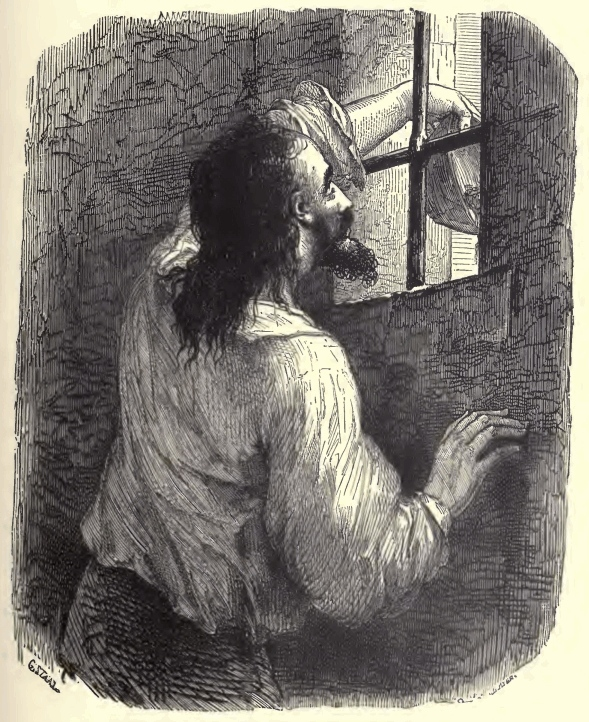
\includegraphics[width=\textwidth]{0185m.jpg}
\end{figure}

Nearly four years had passed away; at the end of the second he had
ceased to mark the lapse of time. Dantès said, “I wish to die,” and had
chosen the manner of his death, and fearful of changing his mind, he
had taken an oath to die. “When my morning and evening meals are
brought,” thought he, “I will cast them out of the window, and they
will think that I have eaten them.”

He kept his word; twice a day he cast out, through the barred aperture,
the provisions his jailer brought him—at first gayly, then with
deliberation, and at last with regret. Nothing but the recollection of
his oath gave him strength to proceed. Hunger made viands once
repugnant, now acceptable; he held the plate in his hand for an hour at
a time, and gazed thoughtfully at the morsel of bad meat, of tainted
fish, of black and mouldy bread. It was the last yearning for life
contending with the resolution of despair; then his dungeon seemed less
sombre, his prospects less desperate. He was still young—he was only
four or five-and-twenty—he had nearly fifty years to live. What
unforseen events might not open his prison door, and restore him to
liberty? Then he raised to his lips the repast that, like a voluntary
Tantalus, he refused himself; but he thought of his oath, and he would
not break it. He persisted until, at last, he had not sufficient
strength to rise and cast his supper out of the loophole. The next
morning he could not see or hear; the jailer feared he was dangerously
ill. Edmond hoped he was dying.

Thus the day passed away. Edmond felt a sort of stupor creeping over
him which brought with it a feeling almost of content; the gnawing pain
at his stomach had ceased; his thirst had abated; when he closed his
eyes he saw myriads of lights dancing before them like the
will-o’-the-wisps that play about the marshes. It was the twilight of
that mysterious country called Death!

Suddenly, about nine o’clock in the evening, Edmond heard a hollow
sound in the wall against which he was lying.

So many loathsome animals inhabited the prison, that their noise did
not, in general, awake him; but whether abstinence had quickened his
faculties, or whether the noise was really louder than usual, Edmond
raised his head and listened. It was a continual scratching, as if made
by a huge claw, a powerful tooth, or some iron instrument attacking the
stones.

Although weakened, the young man’s brain instantly responded to the
idea that haunts all prisoners—liberty! It seemed to him that heaven
had at length taken pity on him, and had sent this noise to warn him on
the very brink of the abyss. Perhaps one of those beloved ones he had
so often thought of was thinking of him, and striving to diminish the
distance that separated them.

No, no, doubtless he was deceived, and it was but one of those dreams
that forerun death!

Edmond still heard the sound. It lasted nearly three hours; he then
heard a noise of something falling, and all was silent.

Some hours afterwards it began again, nearer and more distinct. Edmond
was intensely interested. Suddenly the jailer entered.

For a week since he had resolved to die, and during the four days that
he had been carrying out his purpose, Edmond had not spoken to the
attendant, had not answered him when he inquired what was the matter
with him, and turned his face to the wall when he looked too curiously
at him; but now the jailer might hear the noise and put an end to it,
and so destroy a ray of something like hope that soothed his last
moments.

The jailer brought him his breakfast. Dantès raised himself up and
began to talk about everything; about the bad quality of the food,
about the coldness of his dungeon, grumbling and complaining, in order
to have an excuse for speaking louder, and wearying the patience of his
jailer, who out of kindness of heart had brought broth and white bread
for his prisoner.

Fortunately, he fancied that Dantès was delirious; and placing the food
on the rickety table, he withdrew. Edmond listened, and the sound
became more and more distinct.

“There can be no doubt about it,” thought he; “it is some prisoner who
is striving to obtain his freedom. Oh, if I were only there to help
him!”

Suddenly another idea took possession of his mind, so used to
misfortune, that it was scarcely capable of hope—the idea that the
noise was made by workmen the governor had ordered to repair the
neighboring dungeon.

It was easy to ascertain this; but how could he risk the question? It
was easy to call his jailer’s attention to the noise, and watch his
countenance as he listened; but might he not by this means destroy
hopes far more important than the short-lived satisfaction of his own
curiosity? Unfortunately, Edmond’s brain was still so feeble that he
could not bend his thoughts to anything in particular. He saw but one
means of restoring lucidity and clearness to his judgment. He turned
his eyes towards the soup which the jailer had brought, rose, staggered
towards it, raised the vessel to his lips, and drank off the contents
with a feeling of indescribable pleasure.

He had the resolution to stop with this. He had often heard that
shipwrecked persons had died through having eagerly devoured too much
food. Edmond replaced on the table the bread he was about to devour,
and returned to his couch—he did not wish to die. He soon felt that his
ideas became again collected—he could think, and strengthen his
thoughts by reasoning. Then he said to himself:

“I must put this to the test, but without compromising anybody. If it
is a workman, I need but knock against the wall, and he will cease to
work, in order to find out who is knocking, and why he does so; but as
his occupation is sanctioned by the governor, he will soon resume it.
If, on the contrary, it is a prisoner, the noise I make will alarm him,
he will cease, and not begin again until he thinks everyone is asleep.”

Edmond rose again, but this time his legs did not tremble, and his
sight was clear; he went to a corner of his dungeon, detached a stone,
and with it knocked against the wall where the sound came. He struck
thrice.

At the first blow the sound ceased, as if by magic.

Edmond listened intently; an hour passed, two hours passed, and no
sound was heard from the wall—all was silent there.

Full of hope, Edmond swallowed a few mouthfuls of bread and water, and,
thanks to the vigor of his constitution, found himself well-nigh
recovered.

The day passed away in utter silence—night came without recurrence of
the noise.

“It is a prisoner,” said Edmond joyfully. His brain was on fire, and
life and energy returned.

The night passed in perfect silence. Edmond did not close his eyes.

In the morning the jailer brought him fresh provisions—he had already
devoured those of the previous day; he ate these listening anxiously
for the sound, walking round and round his cell, shaking the iron bars
of the loophole, restoring vigor and agility to his limbs by exercise,
and so preparing himself for his future destiny. At intervals he
listened to learn if the noise had not begun again, and grew impatient
at the prudence of the prisoner, who did not guess he had been
disturbed by a captive as anxious for liberty as himself.

Three days passed—seventy-two long tedious hours which he counted off
by minutes!

At length one evening, as the jailer was visiting him for the last time
that night, Dantès, with his ear for the hundredth time at the wall,
fancied he heard an almost imperceptible movement among the stones. He
moved away, walked up and down his cell to collect his thoughts, and
then went back and listened.

The matter was no longer doubtful. Something was at work on the other
side of the wall; the prisoner had discovered the danger, and had
substituted a lever for a chisel.

Encouraged by this discovery, Edmond determined to assist the
indefatigable laborer. He began by moving his bed, and looked around
for anything with which he could pierce the wall, penetrate the moist
cement, and displace a stone.

He saw nothing, he had no knife or sharp instrument, the window grating
was of iron, but he had too often assured himself of its solidity. All
his furniture consisted of a bed, a chair, a table, a pail, and a jug.
The bed had iron clamps, but they were screwed to the wood, and it
would have required a screw-driver to take them off. The table and
chair had nothing, the pail had once possessed a handle, but that had
been removed.

\begin{figure}[h]
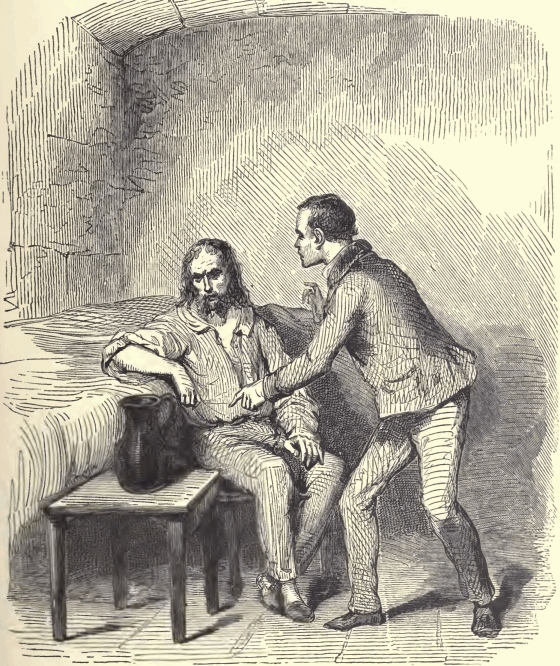
\includegraphics[width=\textwidth]{0189m.jpg}
\end{figure}

Dantès had but one resource, which was to break the jug, and with one
of the sharp fragments attack the wall. He let the jug fall on the
floor, and it broke in pieces.

Dantès concealed two or three of the sharpest fragments in his bed,
leaving the rest on the floor. The breaking of his jug was too natural
an accident to excite suspicion. Edmond had all the night to work in,
but in the darkness he could not do much, and he soon felt that he was
working against something very hard; he pushed back his bed, and waited
for day.

All night he heard the subterranean workman, who continued to mine his
way. Day came, the jailer entered. Dantès told him that the jug had
fallen from his hands while he was drinking, and the jailer went
grumblingly to fetch another, without giving himself the trouble to
remove the fragments of the broken one. He returned speedily, advised
the prisoner to be more careful, and departed.

Dantès heard joyfully the key grate in the lock; he listened until the
sound of steps died away, and then, hastily displacing his bed, saw by
the faint light that penetrated into his cell, that he had labored
uselessly the previous evening in attacking the stone instead of
removing the plaster that surrounded it.

The damp had rendered it friable, and Dantès was able to break it
off—in small morsels, it is true, but at the end of half an hour he had
scraped off a handful; a mathematician might have calculated that in
two years, supposing that the rock was not encountered, a passage
twenty feet long and two feet broad, might be formed.

The prisoner reproached himself with not having thus employed the hours
he had passed in vain hopes, prayer, and despondency. During the six
years that he had been imprisoned, what might he not have accomplished?

This idea imparted new energy, and in three days he had succeeded, with
the utmost precaution, in removing the cement, and exposing the
stone-work. The wall was built of rough stones, among which, to give
strength to the structure, blocks of hewn stone were at intervals
imbedded. It was one of these he had uncovered, and which he must
remove from its socket.

Dantès strove to do this with his nails, but they were too weak. The
fragments of the jug broke, and after an hour of useless toil, Dantès
paused with anguish on his brow.

Was he to be thus stopped at the beginning, and was he to wait inactive
until his fellow workman had completed his task? Suddenly an idea
occurred to him—he smiled, and the perspiration dried on his forehead.

The jailer always brought Dantès’ soup in an iron saucepan; this
saucepan contained soup for both prisoners, for Dantès had noticed that
it was either quite full, or half empty, according as the turnkey gave
it to him or to his companion first.

The handle of this saucepan was of iron; Dantès would have given ten
years of his life in exchange for it.

\begin{figure}[ht]
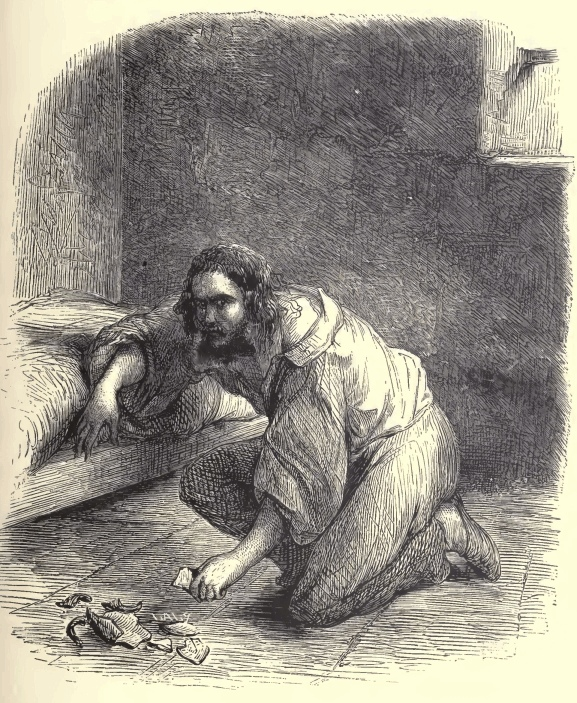
\includegraphics[width=\textwidth]{0191m.jpg}
\end{figure}

The jailer was accustomed to pour the contents of the saucepan into
Dantès’ plate, and Dantès, after eating his soup with a wooden spoon,
washed the plate, which thus served for every day. Now when evening
came Dantès put his plate on the ground near the door; the jailer, as
he entered, stepped on it and broke it.

This time he could not blame Dantès. He was wrong to leave it there,
but the jailer was wrong not to have looked before him. The jailer,
therefore, only grumbled. Then he looked about for something to pour
the soup into; Dantès’ entire dinner service consisted of one
plate—there was no alternative.

“Leave the saucepan,” said Dantès; “you can take it away when you bring
me my breakfast.”

This advice was to the jailer’s taste, as it spared him the necessity
of making another trip. He left the saucepan.

Dantès was beside himself with joy. He rapidly devoured his food, and
after waiting an hour, lest the jailer should change his mind and
return, he removed his bed, took the handle of the saucepan, inserted
the point between the hewn stone and rough stones of the wall, and
employed it as a lever. A slight oscillation showed Dantès that all
went well. At the end of an hour the stone was extricated from the
wall, leaving a cavity a foot and a half in diameter.

Dantès carefully collected the plaster, carried it into the corner of
his cell, and covered it with earth. Then, wishing to make the best use
of his time while he had the means of labor, he continued to work
without ceasing. At the dawn of day he replaced the stone, pushed his
bed against the wall, and lay down. The breakfast consisted of a piece
of bread; the jailer entered and placed the bread on the table.

“Well, don’t you intend to bring me another plate?” said Dantès.

“No,” replied the turnkey; “you destroy everything. First you break
your jug, then you make me break your plate; if all the prisoners
followed your example, the government would be ruined. I shall leave
you the saucepan, and pour your soup into that. So for the future I
hope you will not be so destructive.”

Dantès raised his eyes to heaven and clasped his hands beneath the
coverlet. He felt more gratitude for the possession of this piece of
iron than he had ever felt for anything. He had noticed, however, that
the prisoner on the other side had ceased to labor; no matter, this was
a greater reason for proceeding—if his neighbor would not come to him,
he would go to his neighbor. All day he toiled on untiringly, and by
the evening he had succeeded in extracting ten handfuls of plaster and
fragments of stone. When the hour for his jailer’s visit arrived,
Dantès straightened the handle of the saucepan as well as he could, and
placed it in its accustomed place. The turnkey poured his ration of
soup into it, together with the fish—for thrice a week the prisoners
were deprived of meat. This would have been a method of reckoning time,
had not Dantès long ceased to do so. Having poured out the soup, the
turnkey retired.

Dantès wished to ascertain whether his neighbor had really ceased to
work. He listened—all was silent, as it had been for the last three
days. Dantès sighed; it was evident that his neighbor distrusted him.
However, he toiled on all the night without being discouraged; but
after two or three hours he encountered an obstacle. The iron made no
impression, but met with a smooth surface; Dantès touched it, and found
that it was a beam. This beam crossed, or rather blocked up, the hole
Dantès had made; it was necessary, therefore, to dig above or under it.
The unhappy young man had not thought of this.

“Oh, my God, my God!” murmured he, “I have so earnestly prayed to you,
that I hoped my prayers had been heard. After having deprived me of my
liberty, after having deprived me of death, after having recalled me to
existence, my God, have pity on me, and do not let me die in despair!”

\begin{figure}[ht]
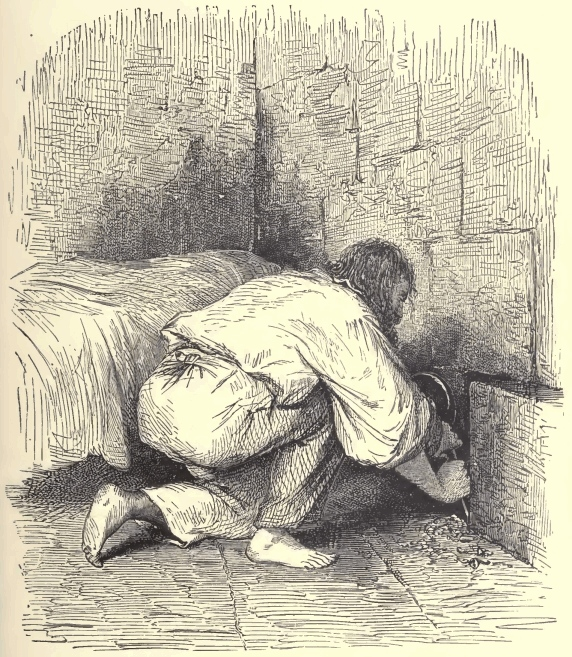
\includegraphics[width=\textwidth]{0193m.jpg}
\end{figure}

“Who talks of God and despair at the same time?” said a voice that
seemed to come from beneath the earth, and, deadened by the distance,
sounded hollow and sepulchral in the young man’s ears. Edmond’s hair
stood on end, and he rose to his knees.

“Ah,” said he, “I hear a human voice.” Edmond had not heard anyone
speak save his jailer for four or five years; and a jailer is no man to
a prisoner—he is a living door, a barrier of flesh and blood adding
strength to restraints of oak and iron.

“In the name of Heaven,” cried Dantès, “speak again, though the sound
of your voice terrifies me. Who are you?”

“Who are you?” said the voice.

“An unhappy prisoner,” replied Dantès, who made no hesitation in
answering.

“Of what country?”

“A Frenchman.”

“Your name?”

“Edmond Dantès.”

“Your profession?”

“A sailor.”

“How long have you been here?”

“Since the 28th of February, 1815.”

“Your crime?”

“I am innocent.”

“But of what are you accused?”

“Of having conspired to aid the emperor’s return.”

“What! For the emperor’s return?—the emperor is no longer on the
throne, then?”

“He abdicated at Fontainebleau in 1814, and was sent to the Island of
Elba. But how long have you been here that you are ignorant of all
this?”

“Since 1811.”

Dantès shuddered; this man had been four years longer than himself in
prison.

“Do not dig any more,” said the voice; “only tell me how high up is
your excavation?”

“On a level with the floor.”

“How is it concealed?”

“Behind my bed.”

“Has your bed been moved since you have been a prisoner?”

“No.”

“What does your chamber open on?”

“A corridor.”

“And the corridor?”

“On a court.”

“Alas!” murmured the voice.

“Oh, what is the matter?” cried Dantès.

“I have made a mistake owing to an error in my plans. I took the wrong
angle, and have come out fifteen feet from where I intended. I took the
wall you are mining for the outer wall of the fortress.”

“But then you would be close to the sea?”

“That is what I hoped.”

“And supposing you had succeeded?”

“I should have thrown myself into the sea, gained one of the islands
near here—the Isle de Daume or the Isle de Tiboulen—and then I should
have been safe.”

“Could you have swum so far?”

“Heaven would have given me strength; but now all is lost.”

“All?”

“Yes; stop up your excavation carefully, do not work any more, and wait
until you hear from me.”

“Tell me, at least, who you are?”

“I am—I am No. 27.”

“You mistrust me, then,” said Dantès. Edmond fancied he heard a bitter
laugh resounding from the depths.

“Oh, I am a Christian,” cried Dantès, guessing instinctively that this
man meant to abandon him. “I swear to you by him who died for us that
naught shall induce me to breathe one syllable to my jailers; but I
conjure you do not abandon me. If you do, I swear to you, for I have
got to the end of my strength, that I will dash my brains out against
the wall, and you will have my death to reproach yourself with.”

“How old are you? Your voice is that of a young man.”

“I do not know my age, for I have not counted the years I have been
here. All I do know is, that I was just nineteen when I was arrested,
the 28th of February, 1815.”

“Not quite twenty-six!” murmured the voice; “at that age he cannot be a
traitor.”

“Oh, no, no,” cried Dantès. “I swear to you again, rather than betray
you, I would allow myself to be hacked in pieces!”

“You have done well to speak to me, and ask for my assistance, for I
was about to form another plan, and leave you; but your age reassures
me. I will not forget you. Wait.”

“How long?”

“I must calculate our chances; I will give you the signal.”

“But you will not leave me; you will come to me, or you will let me
come to you. We will escape, and if we cannot escape we will talk; you
of those whom you love, and I of those whom I love. You must love
somebody?”

“No, I am alone in the world.”

“Then you will love me. If you are young, I will be your comrade; if
you are old, I will be your son. I have a father who is seventy if he
yet lives; I only love him and a young girl called Mercédès. My father
has not yet forgotten me, I am sure, but God alone knows if she loves
me still; I shall love you as I loved my father.”

“It is well,” returned the voice; “tomorrow.”

These few words were uttered with an accent that left no doubt of his
sincerity; Dantès rose, dispersed the fragments with the same
precaution as before, and pushed his bed back against the wall. He then
gave himself up to his happiness. He would no longer be alone. He was,
perhaps, about to regain his liberty; at the worst, he would have a
companion, and captivity that is shared is but half captivity. Plaints
made in common are almost prayers, and prayers where two or three are
gathered together invoke the mercy of heaven.

All day Dantès walked up and down his cell. He sat down occasionally on
his bed, pressing his hand on his heart. At the slightest noise he
bounded towards the door. Once or twice the thought crossed his mind
that he might be separated from this unknown, whom he loved already;
and then his mind was made up—when the jailer moved his bed and stooped
to examine the opening, he would kill him with his water jug. He would
be condemned to die, but he was about to die of grief and despair when
this miraculous noise recalled him to life.

The jailer came in the evening. Dantès was on his bed. It seemed to him
that thus he better guarded the unfinished opening. Doubtless there was
a strange expression in his eyes, for the jailer said, “Come, are you
going mad again?”

Dantès did not answer; he feared that the emotion of his voice would
betray him. The jailer went away shaking his head. Night came; Dantès
hoped that his neighbor would profit by the silence to address him, but
he was mistaken. The next morning, however, just as he removed his bed
from the wall, he heard three knocks; he threw himself on his knees.

“Is it you?” said he; “I am here.”

“Is your jailer gone?”

“Yes,” said Dantès; “he will not return until the evening; so that we
have twelve hours before us.”

“I can work, then?” said the voice.

“Oh, yes, yes; this instant, I entreat you.”

In a moment that part of the floor on which Dantès was resting his two
hands, as he knelt with his head in the opening, suddenly gave way; he
drew back smartly, while a mass of stones and earth disappeared in a
hole that opened beneath the aperture he himself had formed. Then from
the bottom of this passage, the depth of which it was impossible to
measure, he saw appear, first the head, then the shoulders, and lastly
the body of a man, who sprang lightly into his cell.

\begin{figure}[h]
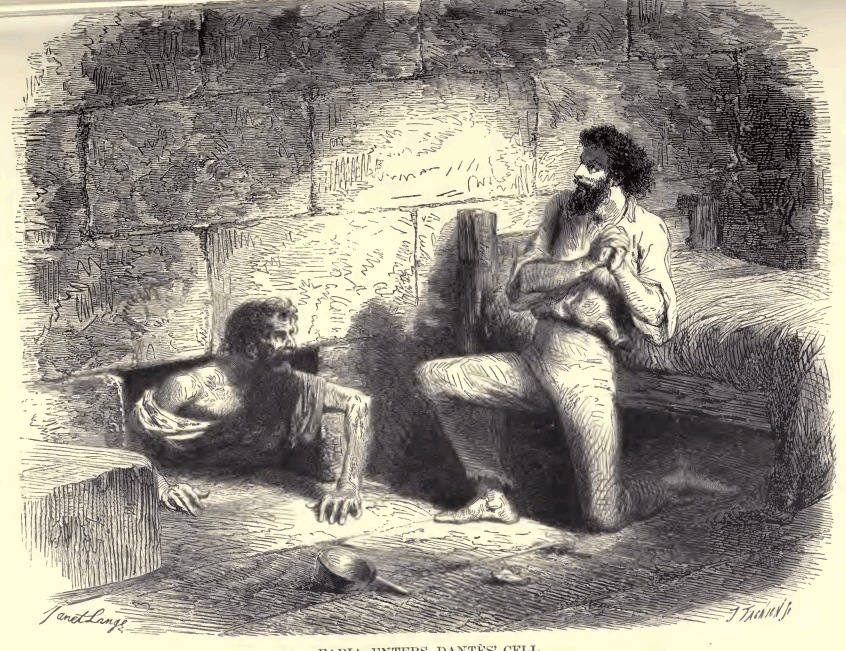
\includegraphics[width=\textwidth]{0197m.jpg}
\end{figure}
